% Created with jtex v.1.0.17
\documentclass{article}
\PassOptionsToPackage{short, nodayofweek}{datetime}


% Start Curvenote Definitions

% Pass Options Section
% base
\PassOptionsToPackage{normalem}{ulem}
\PassOptionsToPackage{utf8}{inputenc}

% template
\PassOptionsToPackage{framemethod=TikZ}{mdframed}
\PassOptionsToPackage{x11names, svgnames}{xcolor}

%%% PACKAGES

% base
\usepackage{inputenc}
\usepackage{url}
\usepackage{graphicx}
\usepackage{adjustbox}
\usepackage{amssymb}
\usepackage{amsfonts}
\usepackage{amsmath}
\usepackage{enumitem}
\usepackage{nicefrac}
\usepackage{booktabs}
\usepackage{microtype}
\usepackage{hyperref}
\usepackage{ulem}
\usepackage{enumitem}
\usepackage{float}
\usepackage{datetime}
\usepackage{xkeyval}
\usepackage{framed}
\usepackage{doi}

% template
\usepackage{natbib}
\usepackage{fancyvrb}
\usepackage{mdframed}
\usepackage{xcolor}

%%%


%%%% Setup Section

% base
\graphicspath{{.}}
% template
\sloppy
\newenvironment{aside}{\begin{framed}}{\end{framed}}
\newmdenv[linewidth=2pt,linecolor=CornflowerBlue,topline=false,bottomline=false,rightline=false,leftline=true,skipabove=20,skipbelow=20,leftmargin=20,rightmargin=20]{callout}
\newfloat{code}{thp}{loc}
\floatname{code}{Program}
\raggedbottom
\bibliographystyle{abbrvnat}
\setcitestyle{authoryear,open={(},close={)},semicolon,aysep={,}}

% End Curvenote Definitions




% colors for hyperlinks
\hypersetup{colorlinks=true, allcolors=blue}
\hypersetup{
pdftitle={\@title},
pdfsubject={},
pdfauthor={\@author},
pdfkeywords={},
addtopdfcreator={Written in Curvenote}
}

\usepackage{curvenote}

\title{Scenario 1}

\newdate{articleDate}{21}{4}{2024}
\date{\displaydate{articleDate}}

\author{\bfseries Hector Nieto\mdseries\\ICA-CSIC\\\AND\bfseries Benjamin Mary\mdseries\\ICA-CSIC\\\AND\bfseries Vicente Burchard-Levine\mdseries\\ICA-CSIC\\}

\begin{document}

\maketitle
\keywords{DA}

\section{Scenario 0}

\subsection{Model}

\begin{itemize}
\item The \textbf{regional domain size} is 100x100m square, flat. \textbf{Irrigation local size} is a 30x30m square centered on the regional domain.
\end{itemize}

\textbf{Soil and Vegetation}

\begin{itemize}
\item The vegetation is uniform on all the regional domain size, with \textbf{root depth} of 1m typical from herbaceous crop.
\item The soil is homogeneous all over the regional domain.
\item \textbf{At time 0}, the soil is dry with an initial pressure head of -30m that is equivalent to a saturation level of 0.3?.
\end{itemize}

\textbf{Atmospheric Boundary conditions}

\begin{itemize}
\item The irrigation consist in a single event at ?? sec (day ??).
\item The irrigation rate is \textbf{5e-07} m/s during \textbf{21600} sec. This is equivalent to 43.2 mm/day during 6hours.
\item The \textbf{potential ETp} is homogeneous all over the domain and with time, set to -1e-07 m/s.
\item \textbf{No flow} boundary conditions are imposed outside the regional domain.
\end{itemize}

\textbf{Observations}

\begin{itemize}
\item Earth Observations are available at a \textbf{daily frequency}.
\end{itemize}

\begin{figure}[!htbp]
\centering
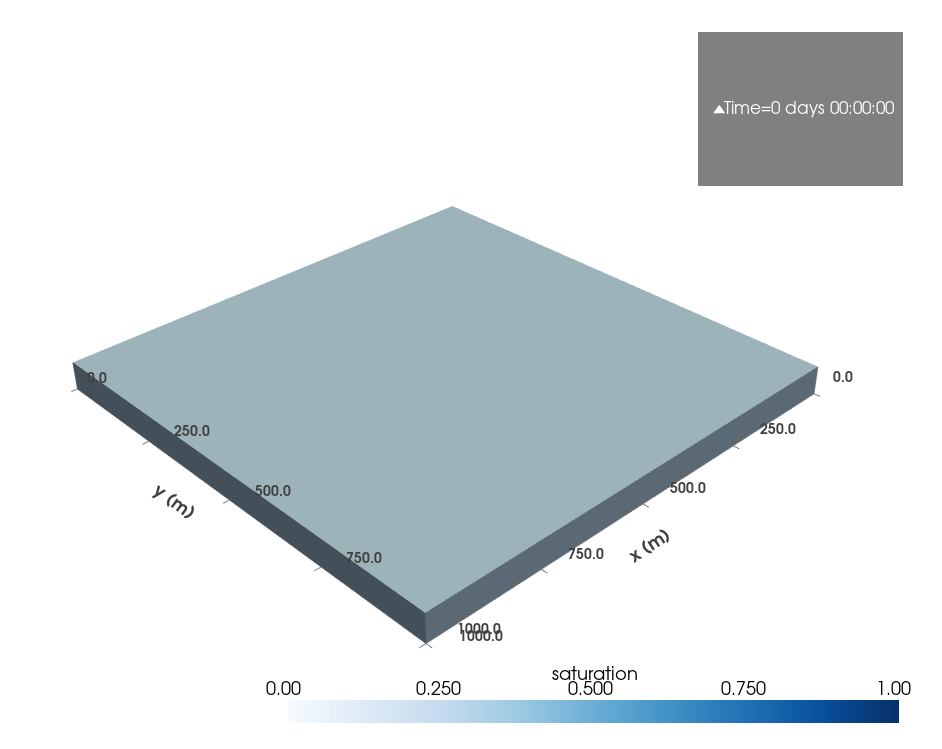
\includegraphics[width=0.75\linewidth]{files/EOMAJI_mesh-509781dd4b086cb32383299dabc9f88d.png}
\caption*{EO-MAJI-IrrDelineation}
\end{figure}

\subsection{Irrigation delimitation}

\begin{figure}[!htbp]
\centering
\includegraphics[width=0.75\linewidth]{files/vtksaturation-6351a4b146f09c4ae6b6fcd05adccf86.gif}
\caption*{Saturation over the course of the irrigation}
\end{figure}

\begin{figure}[!htbp]
\centering
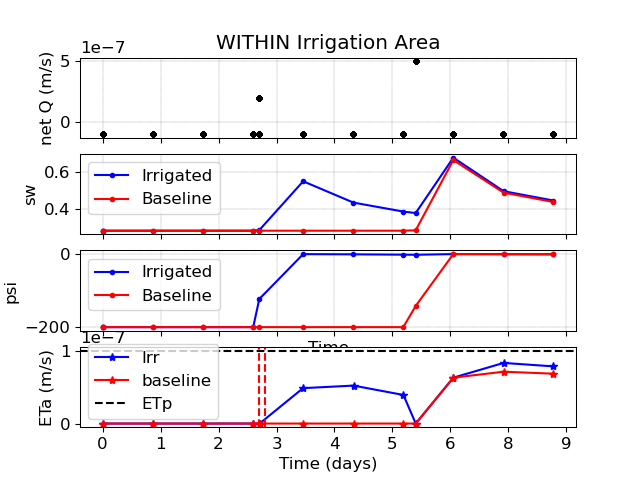
\includegraphics[width=0.875\linewidth]{files/plot_1d_evol_irrArea-219b9fec1dd755590a4d1ac1bb8279bb.png}
\caption*{Scenario 1}
\end{figure}

\begin{figure}[!htbp]
\centering
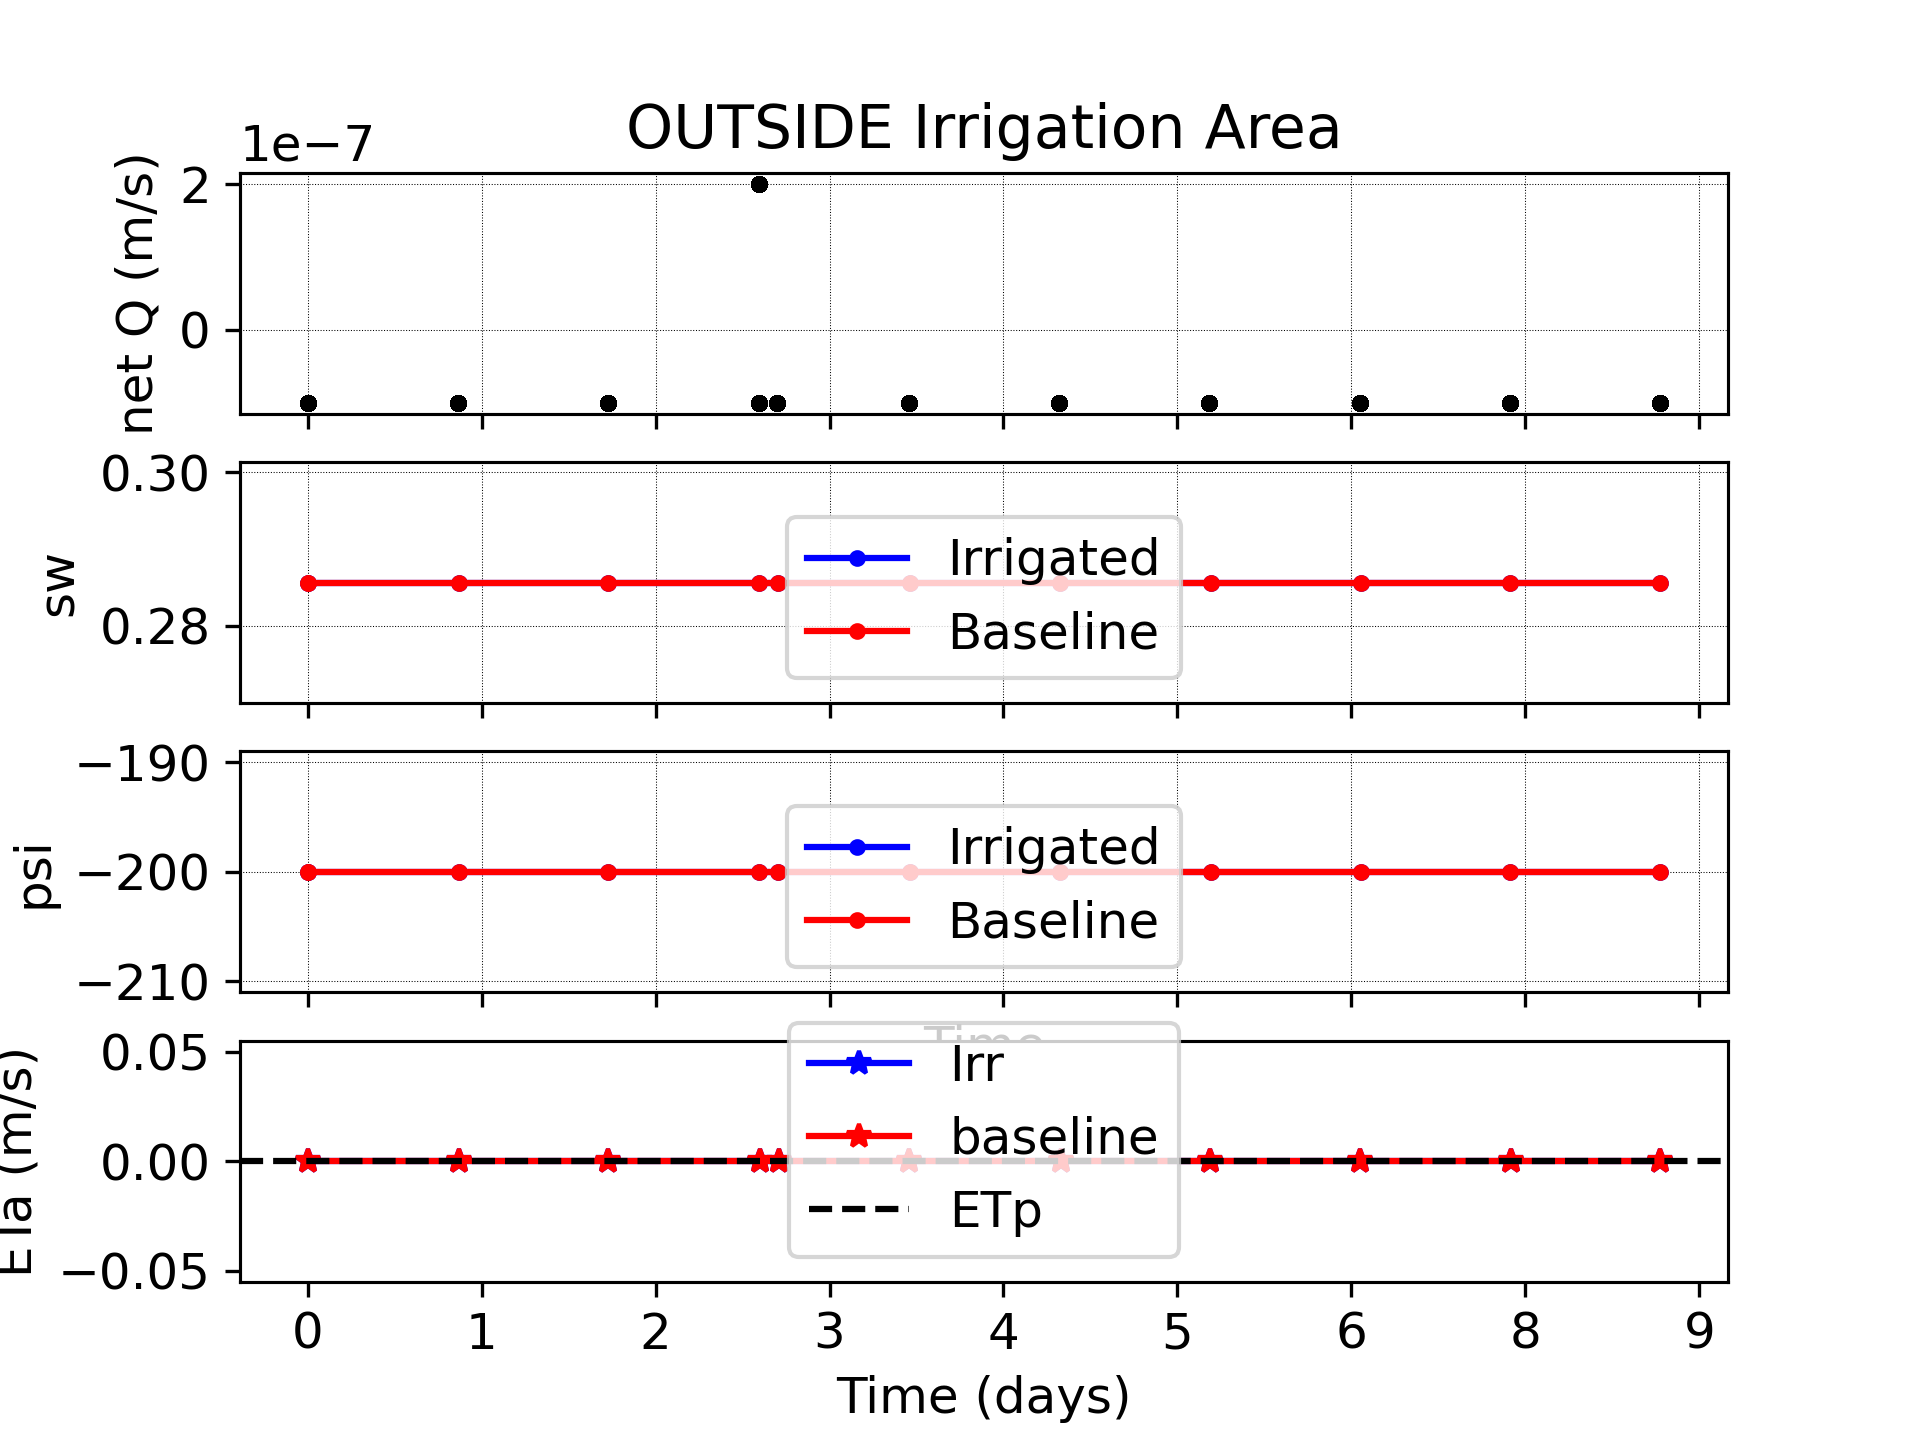
\includegraphics[width=0.875\linewidth]{files/plot_1d_evol_outArea-4651edee791016dd422d335828ba2785.png}
\caption*{SAME AS previous figure but outside the irrigation area.}
\end{figure}

\begin{figure}[!htbp]
\centering
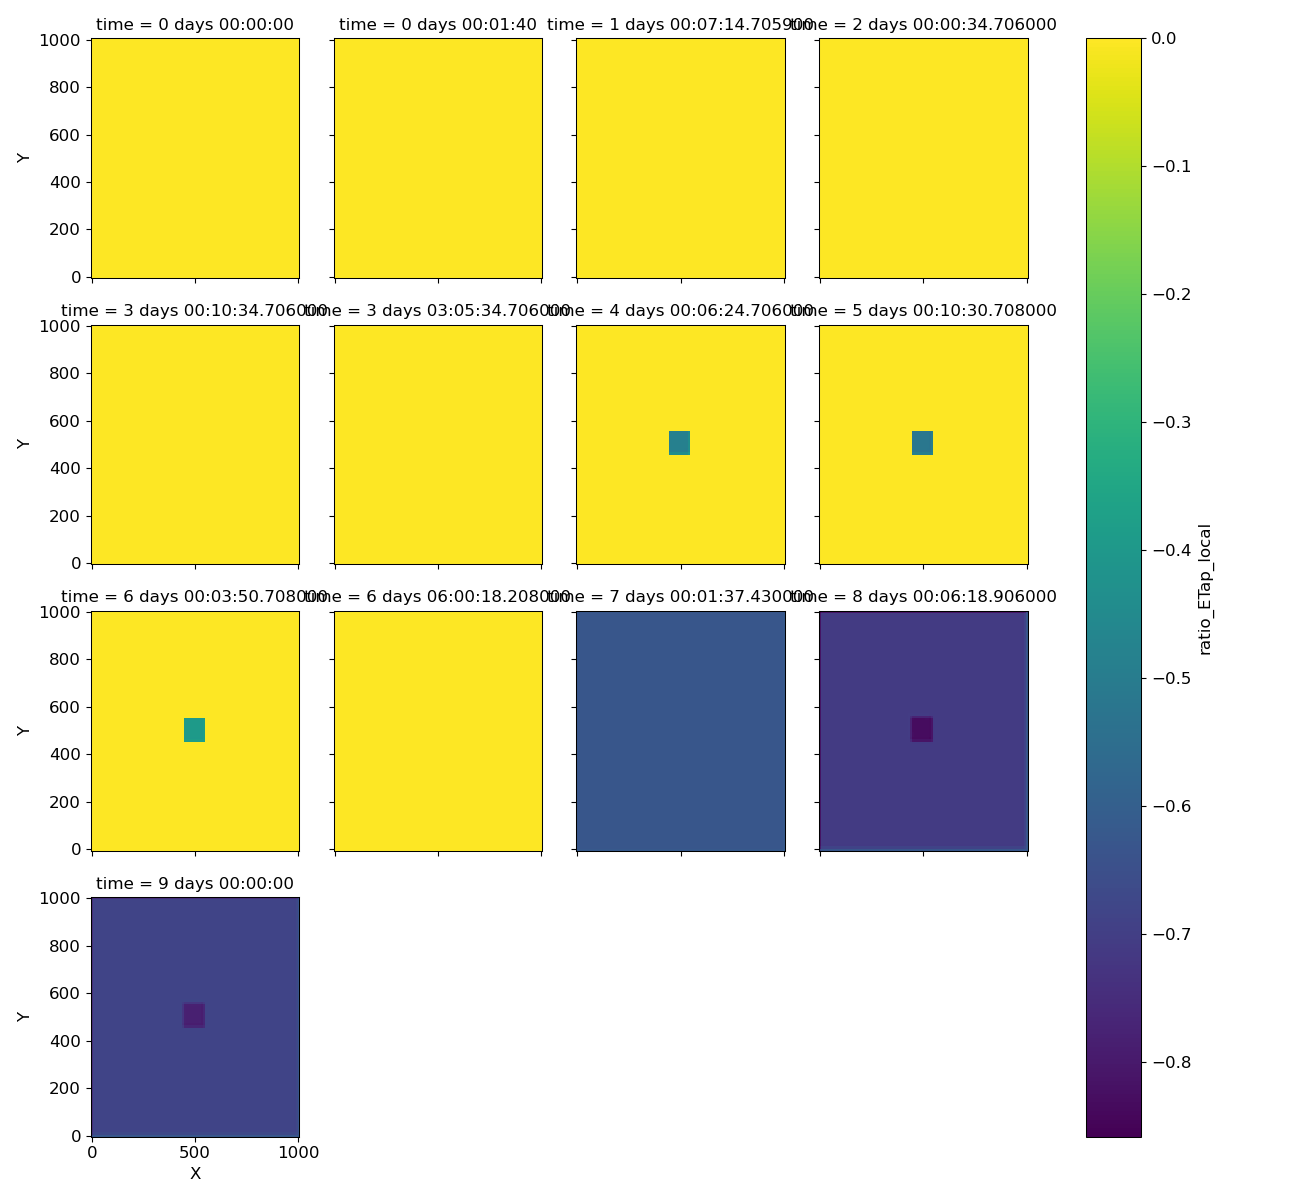
\includegraphics[width=0.875\linewidth]{files/ratioETap_withIRR_sp-3ce82098ed713b0f32abaf56fe476a17.png}
\caption*{For each pixel we compute individually the ratio ETa/ETp.}
\end{figure}

\subsection{Irrigation accounting}

\begin{figure}[!htbp]
\centering
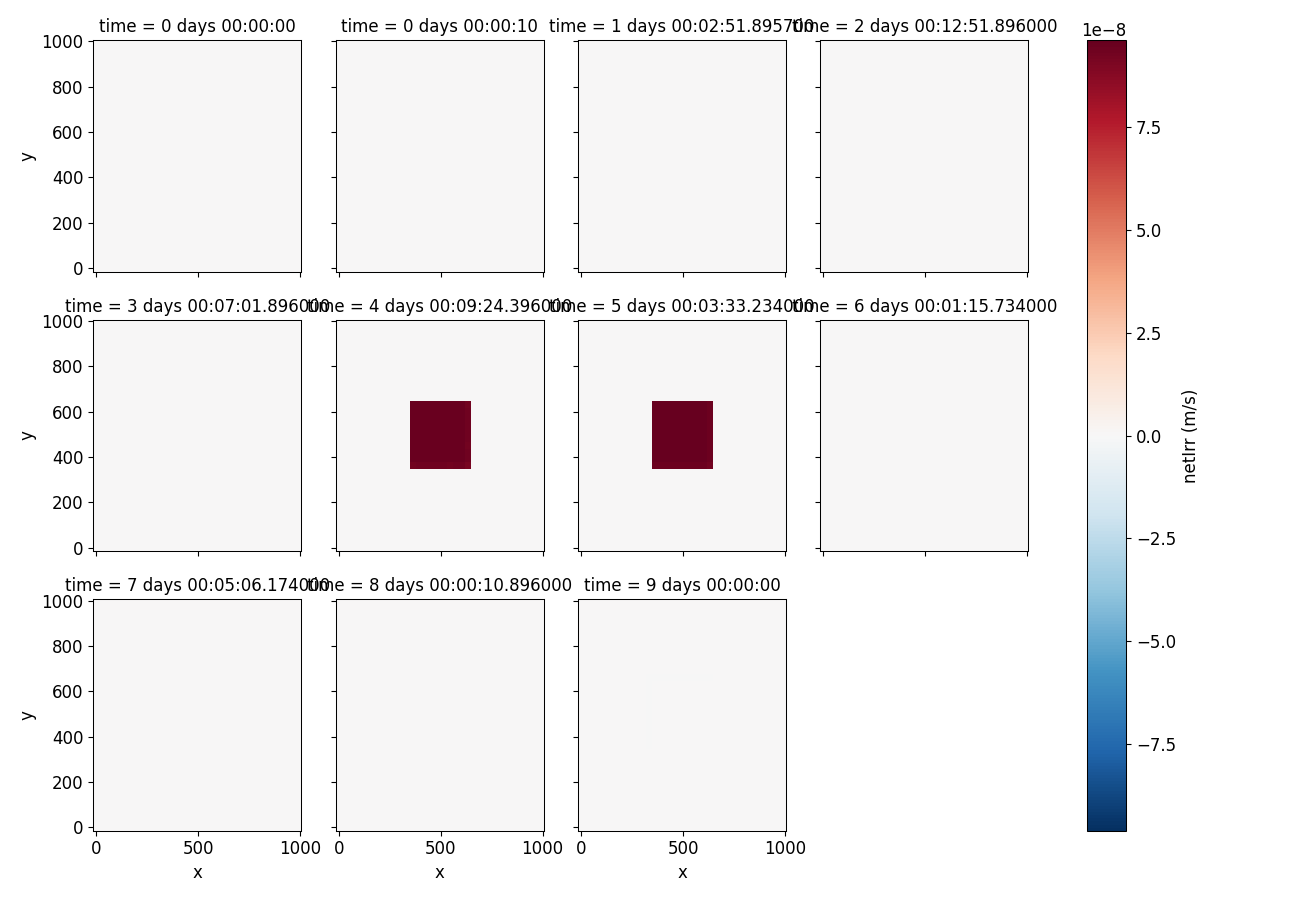
\includegraphics[width=0.875\linewidth]{../figures/scenario1/netIrr_spatial_plot.png}
\caption*{netIrr\_spatial\_plot}
\end{figure}

\begin{figure}[!htbp]
\centering
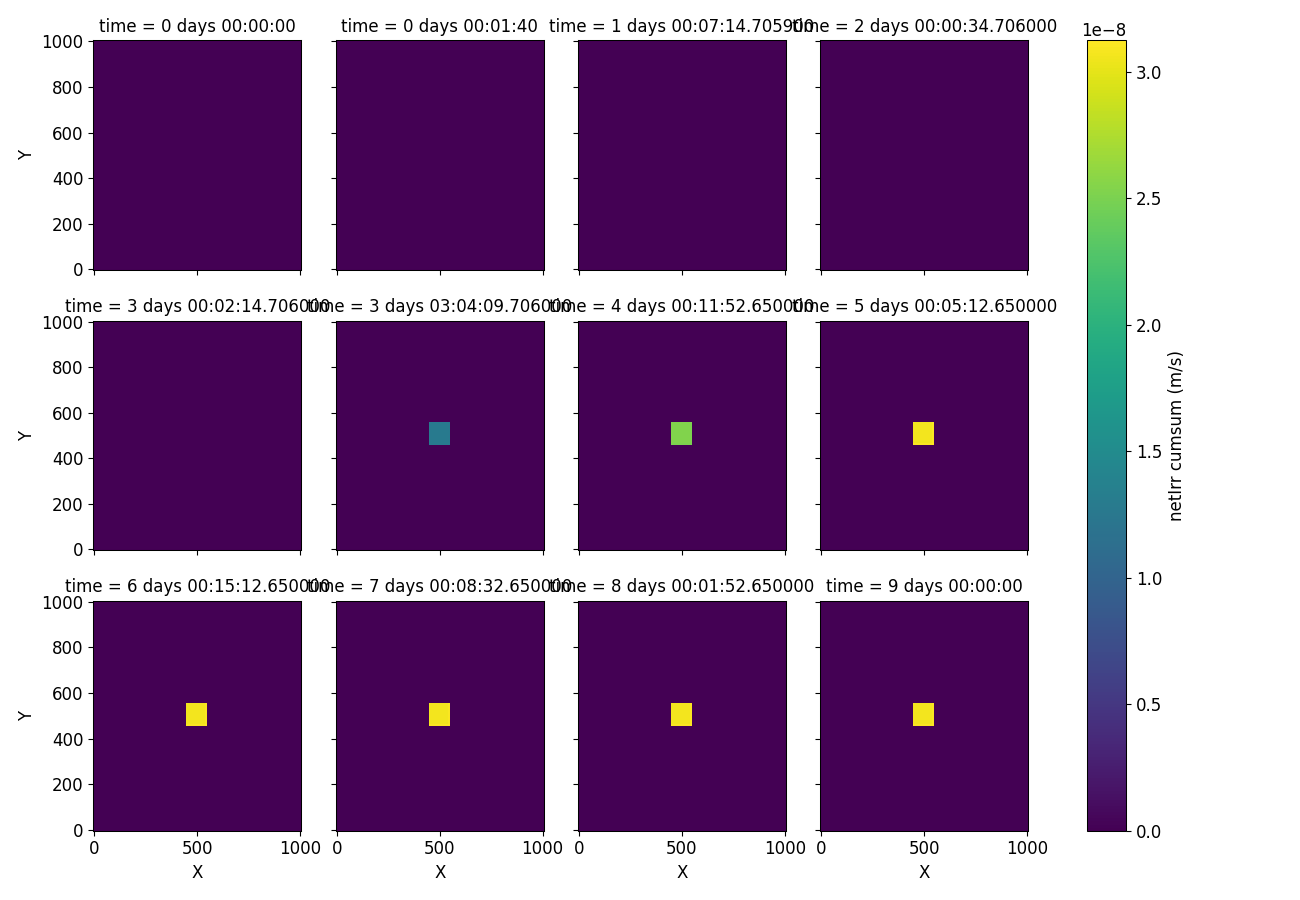
\includegraphics[width=0.875\linewidth]{../figures/scenario1/netIrr_sumsum_spatial_plot.png}
\caption*{netIrr\_sumsum\_spatial\_plot}
\end{figure}

\subsection{Classification \& Decision}
\end{document}
